\section{Experiment Setup}\label{section:exp}

In this section, we discuss the user experiments designed to study and measure the effects of eye contact and gaze in online meetings. 

\subsection{Participants}

We recruited total of 15 participants to partake in our study from our friend-circle and fellow students in the department.
The participants are mostly aged between 18-25 who studies in post-secondary education and all of them are competent in using computers
and other online services such as Zoom. 
We acknowledge the limitation regarding the homogeneity of our sample participants: as it is unclear
how the effects of this technology translates to a more general-represented population.

\subsection{System Requriements}

To run the experiments, we recommend the following system requirements:

\begin{itemize}
    \item \textbf{Operating System}: Windows, macOS, or Linux in 64-bit
    \item \textbf{System Memory}: At least 4 GB
    \item \textbf{CPU}: At least Intel i3 or above
    \item \textbf{GPU}: At least Intel integrated graphics (e.g. Iris Plus Graphics 645) or above
    \item \textbf{Microphone}: yes
    \item \textbf{Zoom}: installed
\end{itemize}

\subsection{Experiments \& Procedures}\label{section:exp-proc}

In this subsection, we outline our preliminary strategy to perform user experiments and collect quantifiable data for our evaluations of how FutureGazer prototype affects user behaviour. We use an existing popular WVC application, Zoom, as our control variable in our experiments. 

We setup FOUR main experiments (1, 2, 3, 4) with varying parameters to test our prototype. Each of the four experiments also has two variants to test the two types of avatar (eyes and heads). The head avatar variant experiments shall have the suffix \textbf{H} and the eye variant of the experiments have \textbf{E}.

Experiment 1 and 2 (E1, E2, H1, H2) involves the participant passively join a meeting. They watch and listen for the visual and audio feedback from the prototype app. We choose to use this experiment to explore \textbf{RQ1}, and study if a person can tell if they're being looked at in an online meeting, and how much.

Experiment 3 (E3, H3) involves involves the participant to speak in a room of mock-avatars. In this case we explore \textbf{RQ3} and attempt to gauge how participants feel, including nervousness, focus, and engagement with the audience using our prototype.

Experiment 4, (E4, H4) involves the participant to join passively as an observer again; 
however, instead of a single presenter speaking (such as in the case with lectures),
the participant watches a conversation. We intend to answer \textbf{RQ2}, and see if with the help
of gaze, participant is more able to identify relationships in a conversations.

For the sake of not being redundant, we do not perform both eye and head variants for experiment 1 and 2. Instead for experiment 1, we only use eye avatar. Similarly, for experiment 2, we only use head avatar. In other words, we \textbf{omit} experiments H1 and E2.

Originally, our plan was to initiate a pop-up window that prompts the test participant to answer whether they think they are being looked at. However, due to complications regards to deploying the prototype executable to people (further complicated by online-only experiments), we decided to aggregate these stare events and ask the test participant questions in the end.

The next subsection outlines the detailed procedures of each of the experiments.

\subsubsection{Experiment E1}

\begin{figure}
     \centering
     \begin{subfigure}[b]{0.3\textwidth}
         \centering
         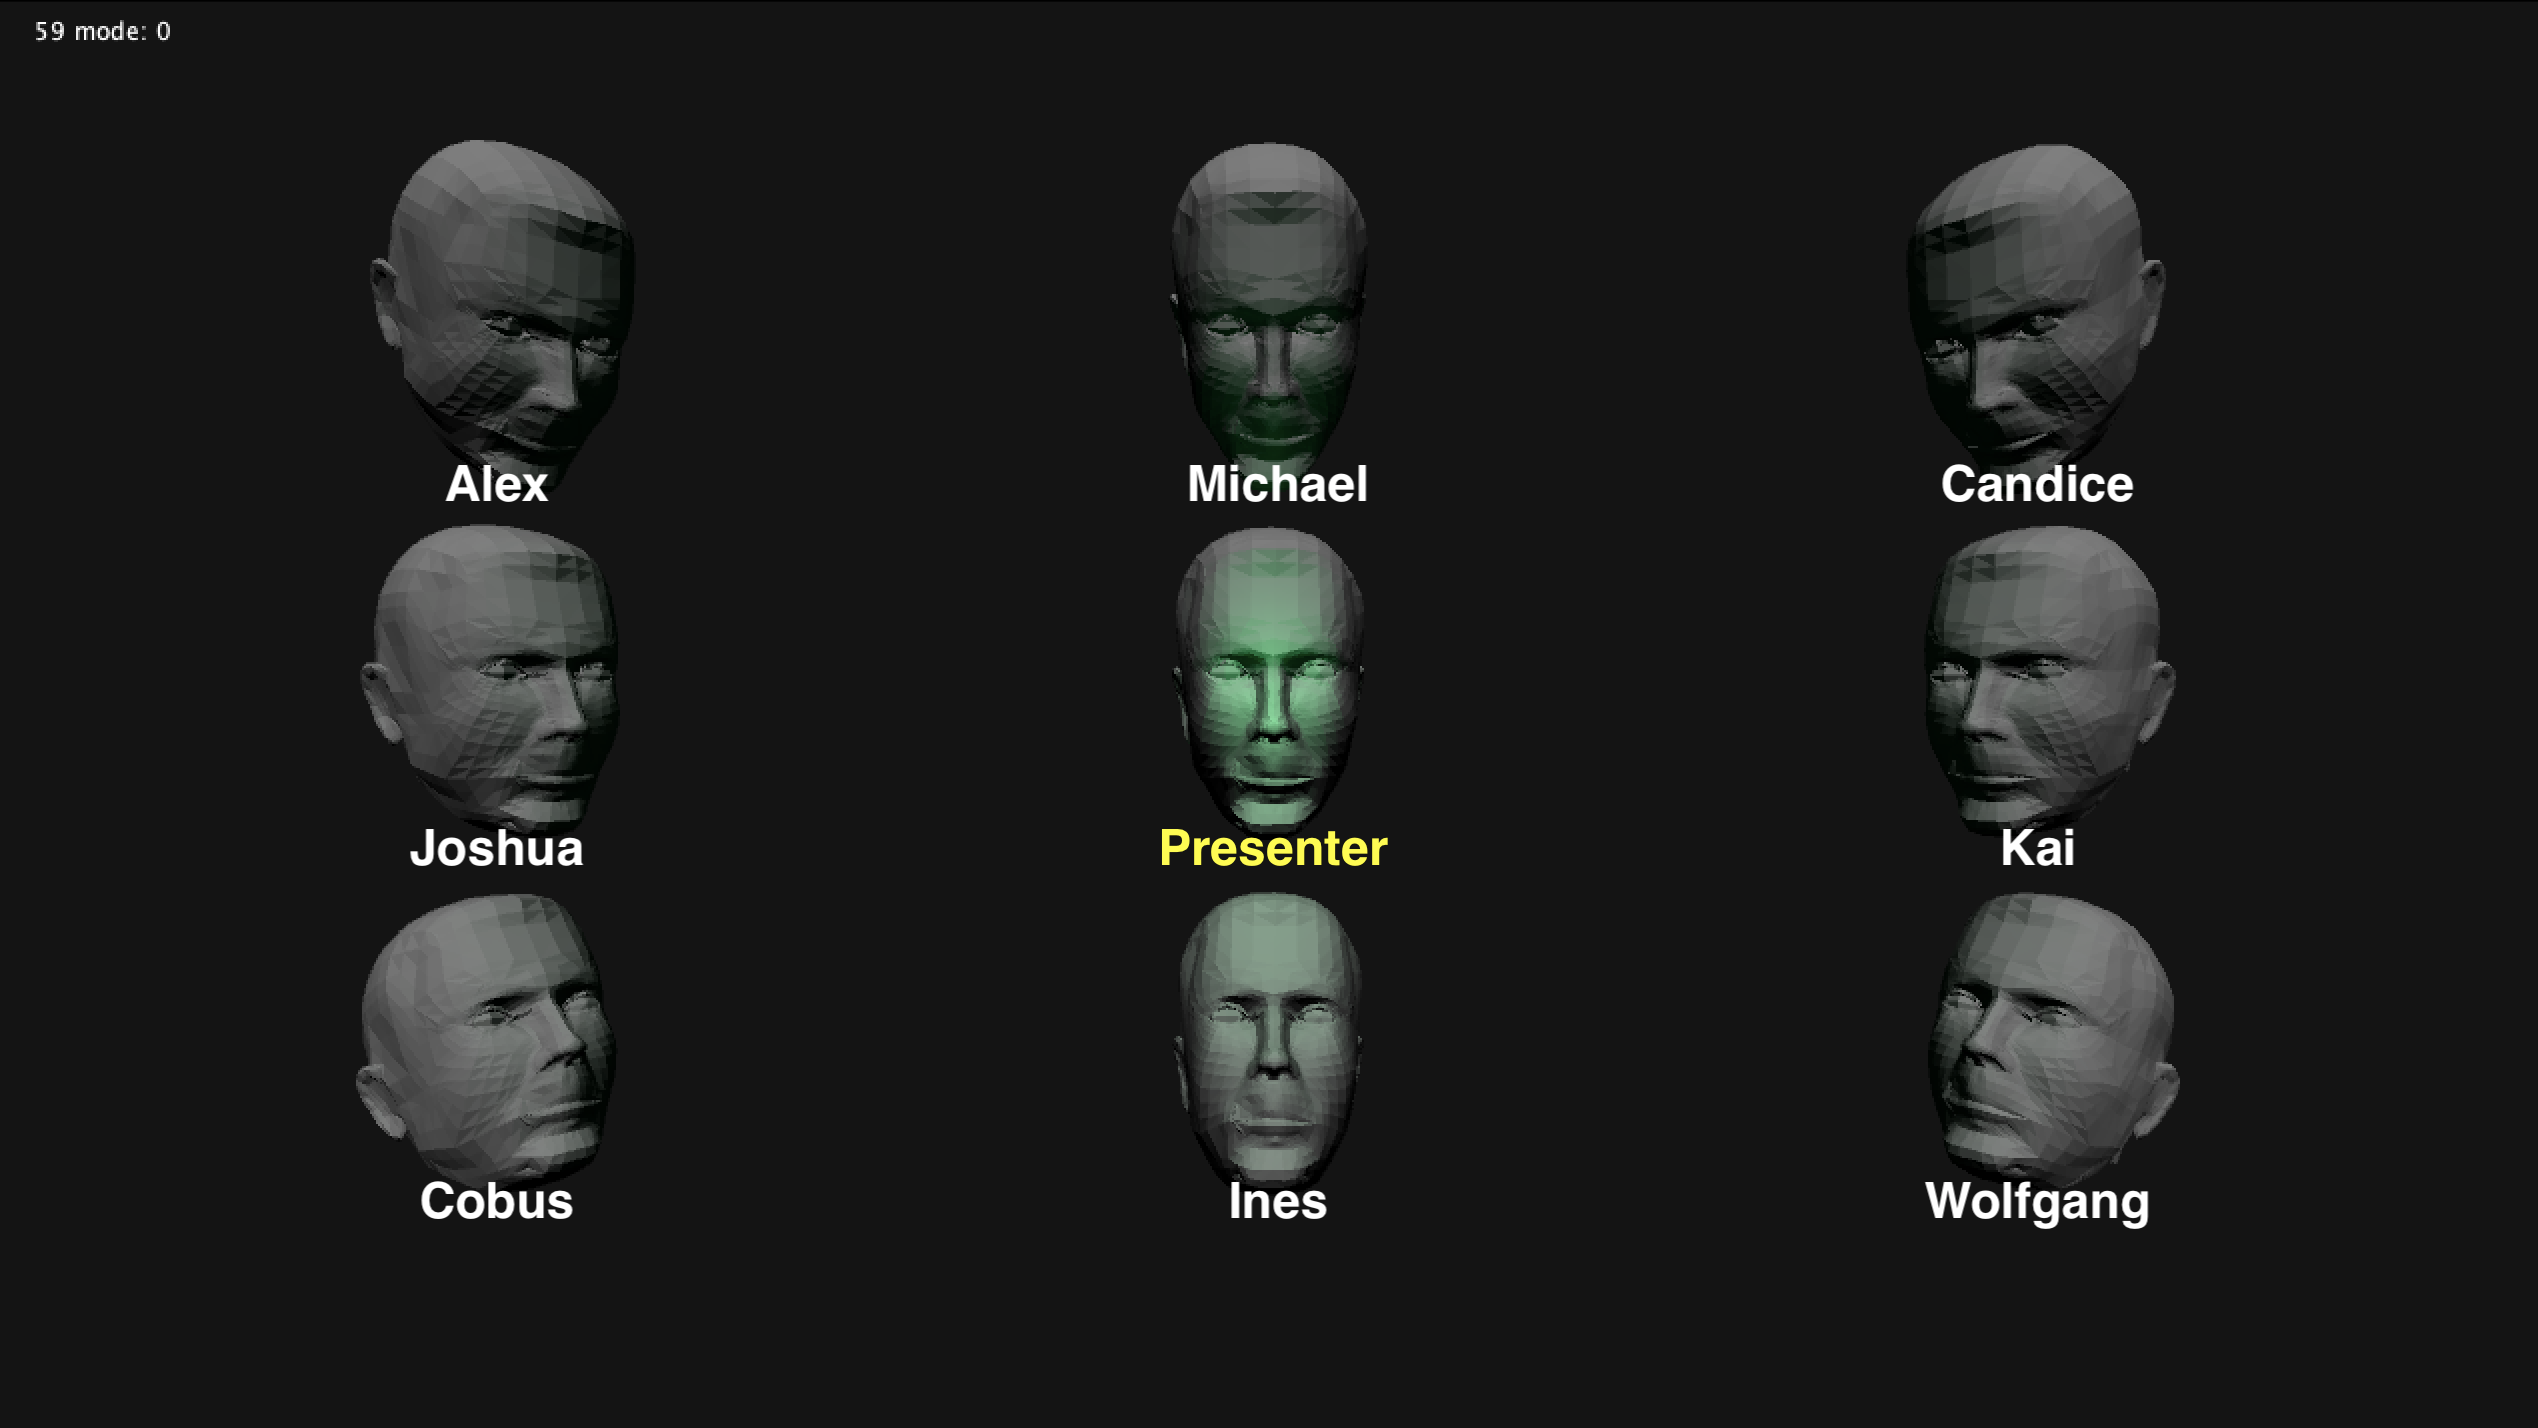
\includegraphics[width=\textwidth]{expA-1.png}
         \caption{}
     \end{subfigure}
     ~
     \begin{subfigure}[b]{0.3\textwidth}
         \centering
         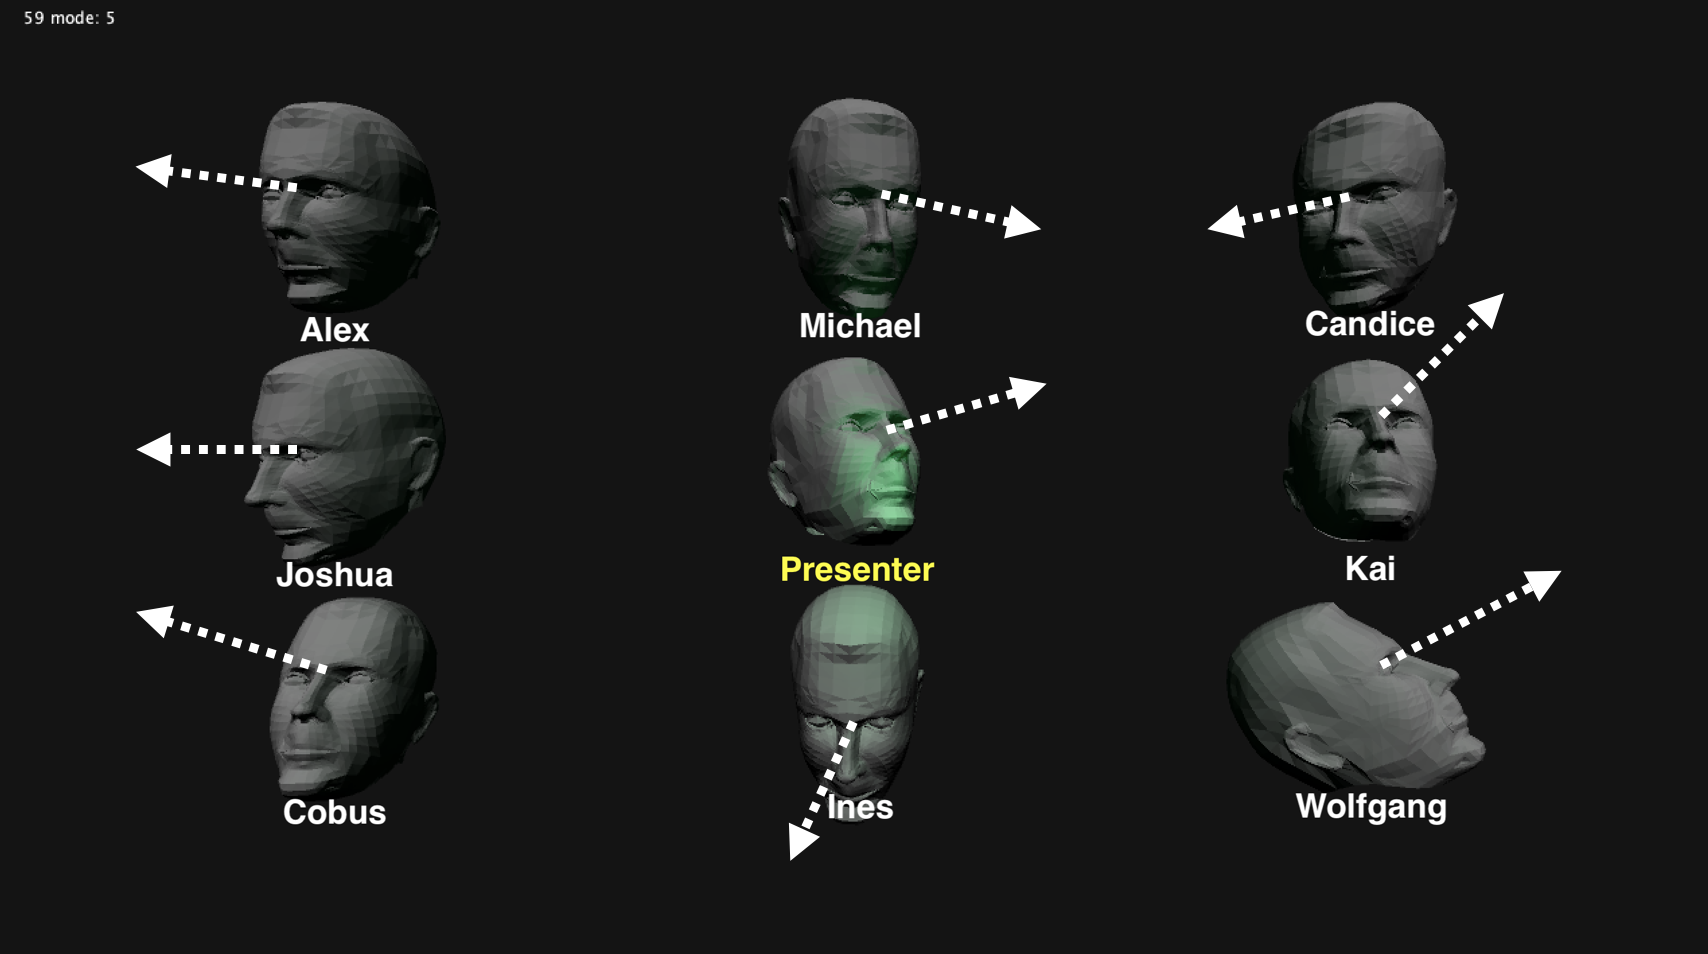
\includegraphics[width=\textwidth]{expA2.png}
         \caption{}
     \end{subfigure}
     ~
     \begin{subfigure}[b]{0.3\textwidth}
         \centering
         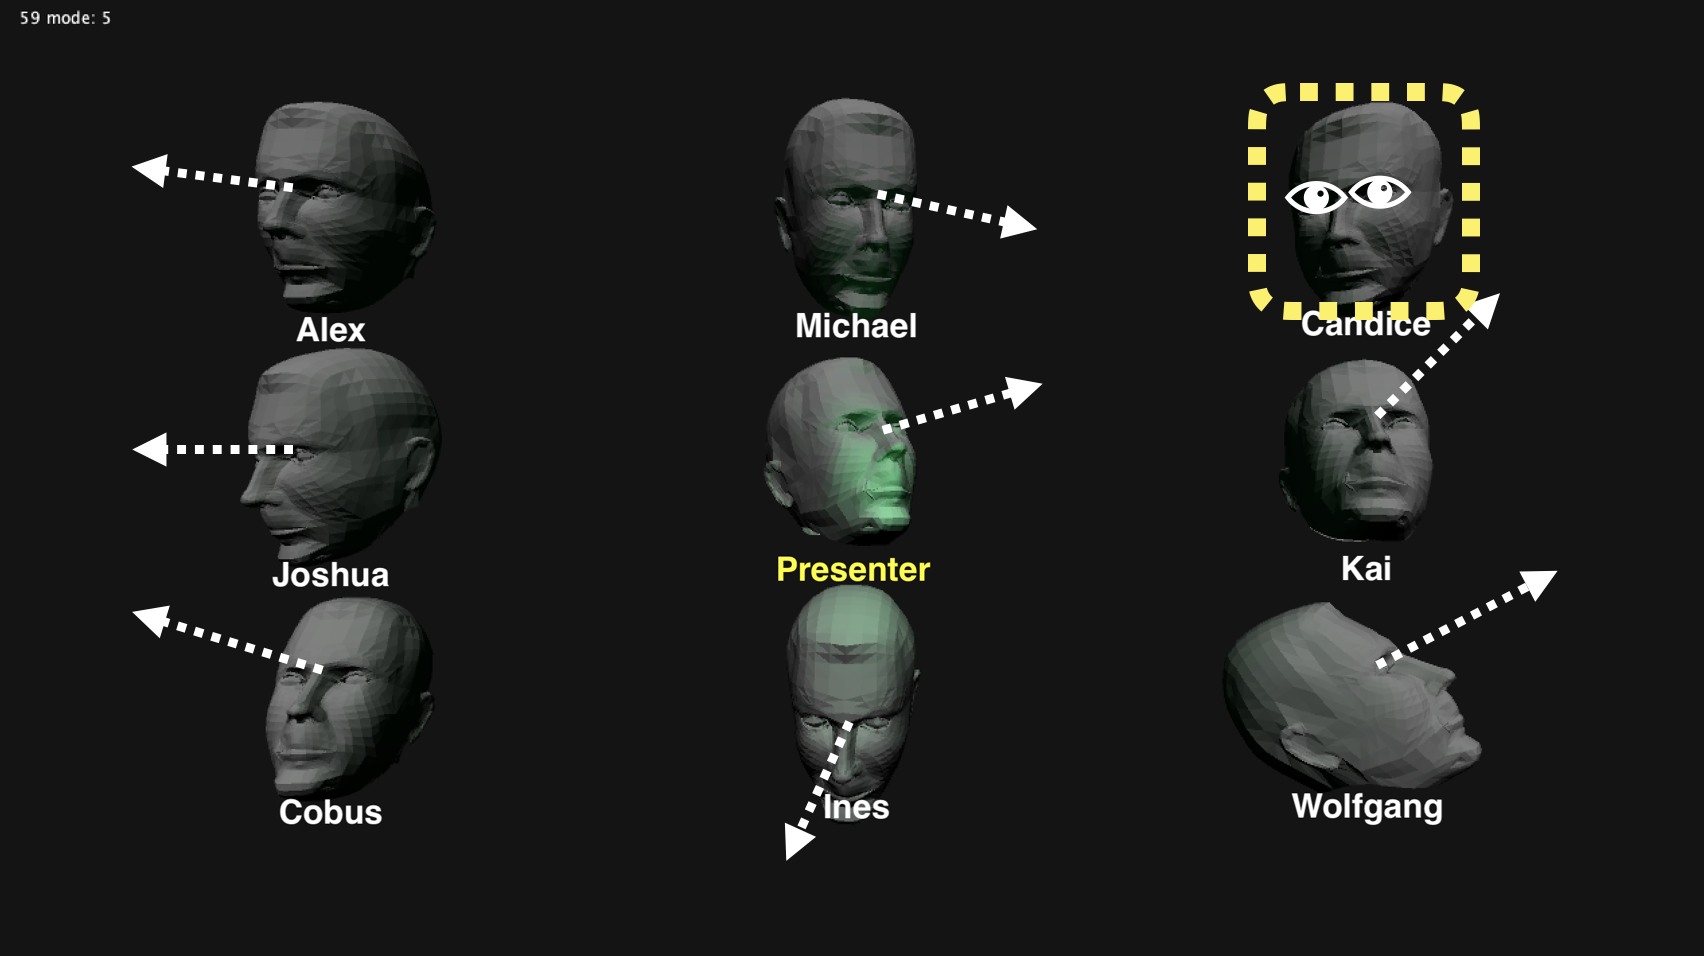
\includegraphics[width=\textwidth]{expA3.png}
         \caption{}
     \end{subfigure}
    \caption{(a) The initialized WVC meeting room with eight mock-avatars including a presenter-avatar. (b) All avatars programmed to look into random directions. (c) Selected mock-avatars would occasionally execute ``stare" where they look out of the screen and towards the participant. Note the dashed lines are for visualization only and cannot be seen by the participant.}
    \label{fig:expa}
\end{figure}

Begin by setting up nine mock-avatars in the WVC window, each with a unique name as seen in Figure \ref{fig:expa}(a). The mock-avatars does not correspond to real users in the WVC room and are programmed and controlled prior to user testing. Note that in Figure \ref{fig:expa}, head avatars are used, but as mentioned in \ref{section:exp-proc}, only eye avatars are used for experiment A.

The test participant joins the meeting session as the tenth person --- who is not visible on the screen. Initially, the mock-avatars move randomly for several seconds (Figure \ref{fig:expa}(b)). Meanwhile an audio track of a lecture or a podcast plays.
One of the mock-avatar, hereafter called \textit{presenter-avatar}, is programmed to be synced with the audio track for the sake of realism.
Throughout the meeting, a set of specific pre-programmed mock-avatars (that is not the presenter-avatar) will look at the test participant (look out from the screen) intermittently for several seconds at varying frequencies without disrupting the presenter-avatar or the audio (Figure \ref{fig:expa}(c)). We call this event a stare. The participant does not know which mock-avatars are selected to look at them before the experiment to preserve the validity of the results.

Finally we compare and correlate the participants’ response, such as perceived number of gazes
(avatars that ``stared" for longer than 3 seconds), glimpses (avatars that ``stared for less than 3 seconds). We compare their response with the ground truth which is logged in the prototype application. The correlation tests the hypothesis set in RQ1.

\subsubsection{Experiment H2}

Experiment B explores RQ3 by observing whether a person who is paying attention to a presenter can notice another person who starts to look at them (i.e. the gaze target change to the subject).

The procedure is identical to experiment E1, and as mentioned in Section \ref{section:exp-proc}, this experiment is only performed using 3D heads as avatars.
At the end of the experiment, we ask the participant the same question as experiment A.
Additionally, we ask how the experience differs from experiment E1 --- in particular, 
how much more attention has the heads garnered compared to experiment E1.

% \paragraph{External Tracking Variation}

% In the original design of Experiment B, we prompt the participants with a line of text to ask them to click. However, this might cause bias as doing so primes the participants with extra hints that affect experiment output. Thus, the variation of Experiment B, called Experiment B-TCK, uses an external gaze tracking system to measure where the participant is looking at. 

% In Experiment B-TCK, the mock-avatar setup is identical to Experiment B, except the preprogrammed stare event sequences are predetermined/logged. We use external gaze tracking systems such as tobii [9] to log participants’ actual gaze target instead of relying on the participants to actively click on the mock-avatar they think that is looking at them. For evaluation, we compare and correlate the predetermined gaze sequence of the mock-avatars with the captured gazes of the participants’ throughout the experiment. We hypothesize that during the first  seconds, the participant mostly focuses on A, but as B initiates a stare, we expect the participant to shift their gaze to B’s location on the screen.

% However, due to COVID-19 pandemic remote work requirement of this project, we do not expect to carry-out Experiment B-TCK. 

\subsubsection{Experiment E3, H3}

In E3 and H3, we attempt to test whether the presenter can tell if the audience is paying attention to their speech and tackles both RQ1 and RQ3.

We first ask the participant to observe a short film or review a concept they would like to talk about. Once they're ready, We set up five mock-avatars in the WVC window and the participant will join the session as the sixth user.
The participant will then summarize the short film, or talk about a concept for one to two minutes while the mock-avatars are looking at the participant.
Each of the mock-avatars can randomly toggle between two modes: Paying attention (PA) and Not paying attention (NPA). During the experiment, we program the prototype app such that random mock-avatars is selected and it can toggle between PA and NPA modes at random times. These events are generated/logged for us to compare with.

After the participants are done talking, we ask the participant to rate whether they think they are being paying attention to, based on how many avatars they think that is paying attention. 
We also assess participants' nervousness, focus, and engagement level as they were speaking throughout the session. The participants report these as a rating from 0 to 100\% \textit{compared to} as if they were to perform the same task using traditional WVC apps such as Zoom.

In the end we compare the participants’ observations of how many mock-avatars are paying attention versus the logged values. A strong correlation implies that RQ1 and RQ3 are likely true. We also aggregate the response data and observe effects on the participants as presenters.

We repeat the process for the other avatar type.

\subsubsection{Experiment E4, H4}

In experiments E4, H4, we attempt to test RQ2 in a small-group WVC environment as we assume eye contact amongst two or more people can incite a closer and intimate relationship to an observer \cite{RN10}. Inspired by the body sheets as a method to collect user responses in La Delfa et al.’s work in Drone Chi \cite{RN49}, we intend to use a relationship matrix sheet to study the effect of 3D avatars in

We set up four mock-avatars talking to and looking at each other with a pre-programmed sequence
along with pre-recorded audio.

Each mock-avatar take turns talking. Meanwhile, the other three mock-avatars who are not talking will look at the avatar who is talking.
Occasionally and randomly, the non-presenting avatars can choose to look at another avatar, but not the participant.
Thus, we can describe the engagement and interaction between the four avatars as a relationship matrix:

\begin{equation*}
\mathbf P = \begin{bmatrix}
0 & p_{a,b} & p_{a,c} & p_{a,d} \\ 
p_{b,a} & 0 & p_{b,c} & p_{b,d} \\ 
p_{c,a} & p_{c,b} & 0 & p_{c,d} \\ 
p_{d,a} & p_{d,b} & p_{d,c} & 0 \\ 
\end{bmatrix}
\end{equation*}

Where $p_{a,b}$ is the probability mock-avatar $a$ is looking at/paying attention to $b$ and all columns and rows adds up to 1.0. 

When the experiment is complete and all mock-avatars finished taking turns speaking, we give the relationship matrix as shown in Figure \ref{fig:relmatrix} to the participant to articulate which avatar-pair is more intimate, as well as which avatar is talking with which.
Evaluation: 

We ask the participants to mark each directional arrow, as shown in Figure \ref{fig:relmatrix}, of the relationship matrix, to indicate which avatar is engaging with which. We may also ask the participant to annotate each arrow with a confidence score (0.0 - 1.0). These scores can be normalized and compared with the probability matrix $\mathbf P$ that was pre-programmed into the mock-avatars. A strong correlation of participants’ response and  would imply RQ2 is likely true.

We repeat the process for the other avatar type.

\begin{figure}
	\centering
 	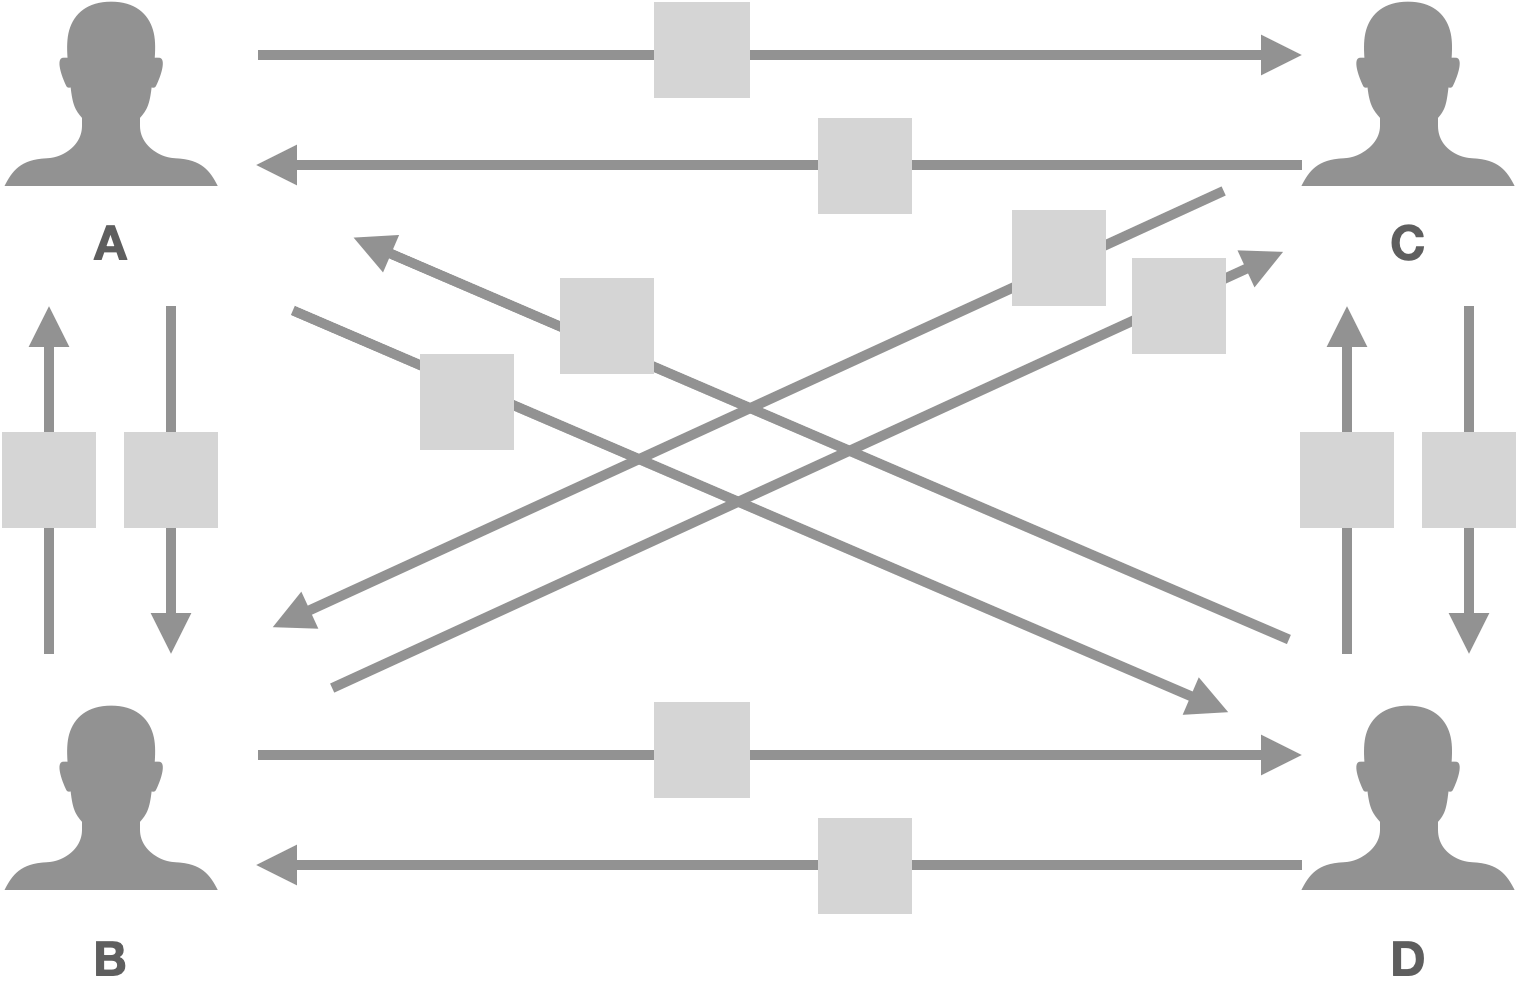
\includegraphics[width=0.7\textwidth]{relmatrix.png}
	\caption{The diagram we ask the participant to fill out which corresponds to the relationship matrix $\mathbf P$}
	\label{fig:relmatrix}
\end{figure}


%%%%%%%%%%%%%%%%%%%%%%%%%% END OF EXPERIMENT DESGIN SECTION
